\section{Work Efficiency Metric} \label{sec:metric}

    In this section we define work efficiency, a metric for comparing different optimized versions of a program when executing with
    different inputs. We define it as the ratio between the amount of \textit{work}, $\Delta W$, performed during a period of time, $\Delta
    t$.

    \[
       \textrm{Work Efficiency} = \frac{\Delta W}{\Delta t}
    \]

    The main challenge is to precisely define what represents \textit{work}. We define the work done by a program on an input to be the
    time taken by the unoptimized program to process that input. We estimate the runtime of each instruction type and then work is the sum
    of the runtime for each instruction type multiplied by its dynamic count.

    \[ \Delta W = \sum_i w_i.n_i \]

    Where $i$ is the instruction type; $w_i$ is the estimated runtime for instruction type $i$; and $n_i$ is the number of observed
    executions of instruction type $i$.

    Similarly to previous work~\citep{giusto01,powell09,brandolese11}, the coefficients, $w_i$, are estimated by linear regression. We create
    one regressor data point for each of a set of program and input pairs.
    We use a separate set of programs from those discussed in Sections~\ref{sec:setup} and \ref{sec:results}.
    %for estimating the architectural settings for the work metric.
    The response variable is the execution time of the unoptimized program as it processes the input. To ensure
    statistically sound results, the execution time is measured by repeated execution until the 99\% confidence interval is no larger than 1\% of
    the mean. The explanatory variables are the dynamic instruction counts for each program and input pair. They are recorded by a separate,
    instrumented run of the program on the input.

    Figure~\ref{fig:work-vs-O0time} shows the correlation of the work metric ($\Delta W$) with runtime on instances of the unoptimized \texttt{susan\_c} benchmark.
    Each point represents the execution of a single input, from a total of 1,000 inputs.
    The correlation coefficient is $0.99$, and the mean absolute percentage error (MAPE) is only about 3.5\%.
    This result suggests that the new efficiency metric correlates much better with speedup than either execution time or IPC.

    %Figure~\ref{fig:motivation-work-efficiency} shows a similar plot to Figure~\FIXME{\ref{fig:motivation-metric}},
    %of work efficiency versus speedup for 500 different binaries of \texttt{susan\_c}.
    %Here the new metric correlates much better than either execution time or IPC,
    %exhibiting a correlation coefficient of $0.93$ with speedup.

    \begin{figure}[t]
        \centering
        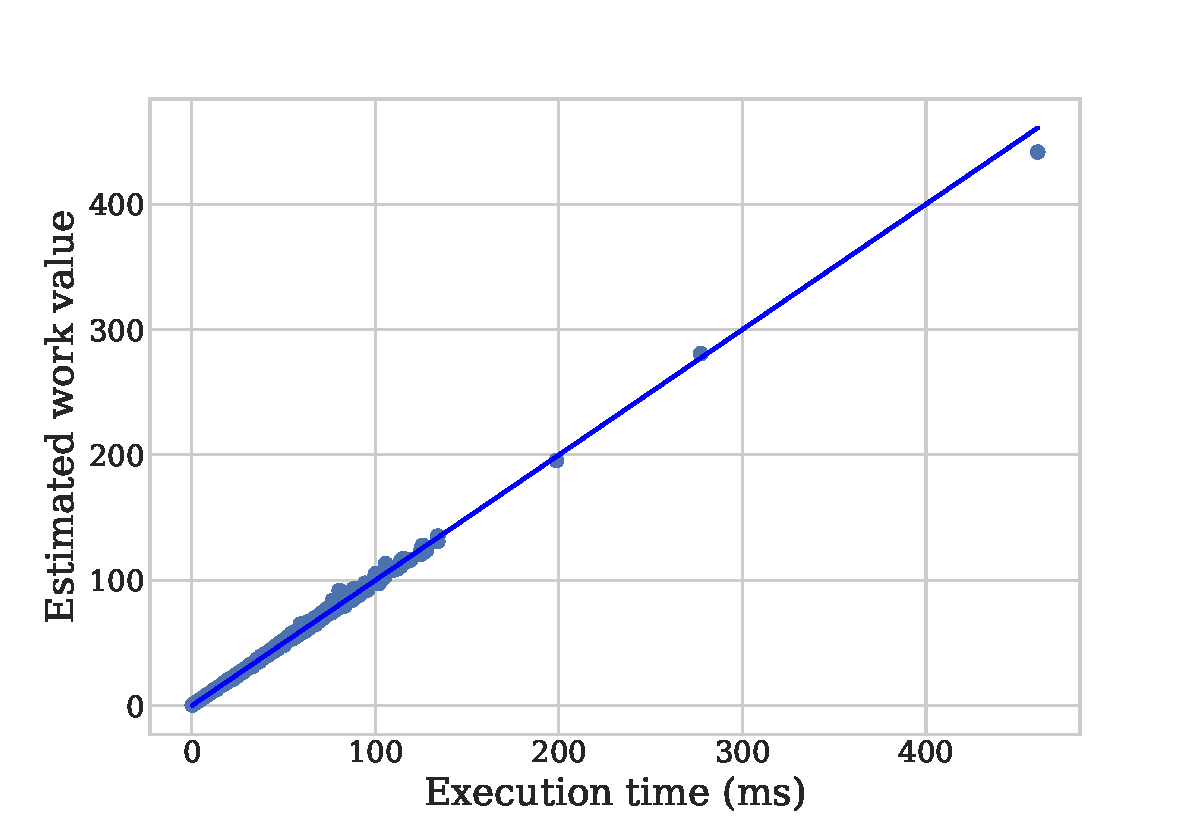
\includegraphics[width=0.5\textwidth]{figs/work-correlation-with-O0_susan_c.pdf}
        \caption{
            Relationship between work metric ($\Delta W$) and the execution time
            of the unoptimized version of the \texttt{susan\_c} benchmark over the
            1,000 inputs.
            Each point represents the execution of a single input.
            They have a correlation coefficient of $0.99$.
        }
        \label{fig:work-vs-O0time}
    \end{figure}

    %\begin{figure}[t]
    %    \centering
    %    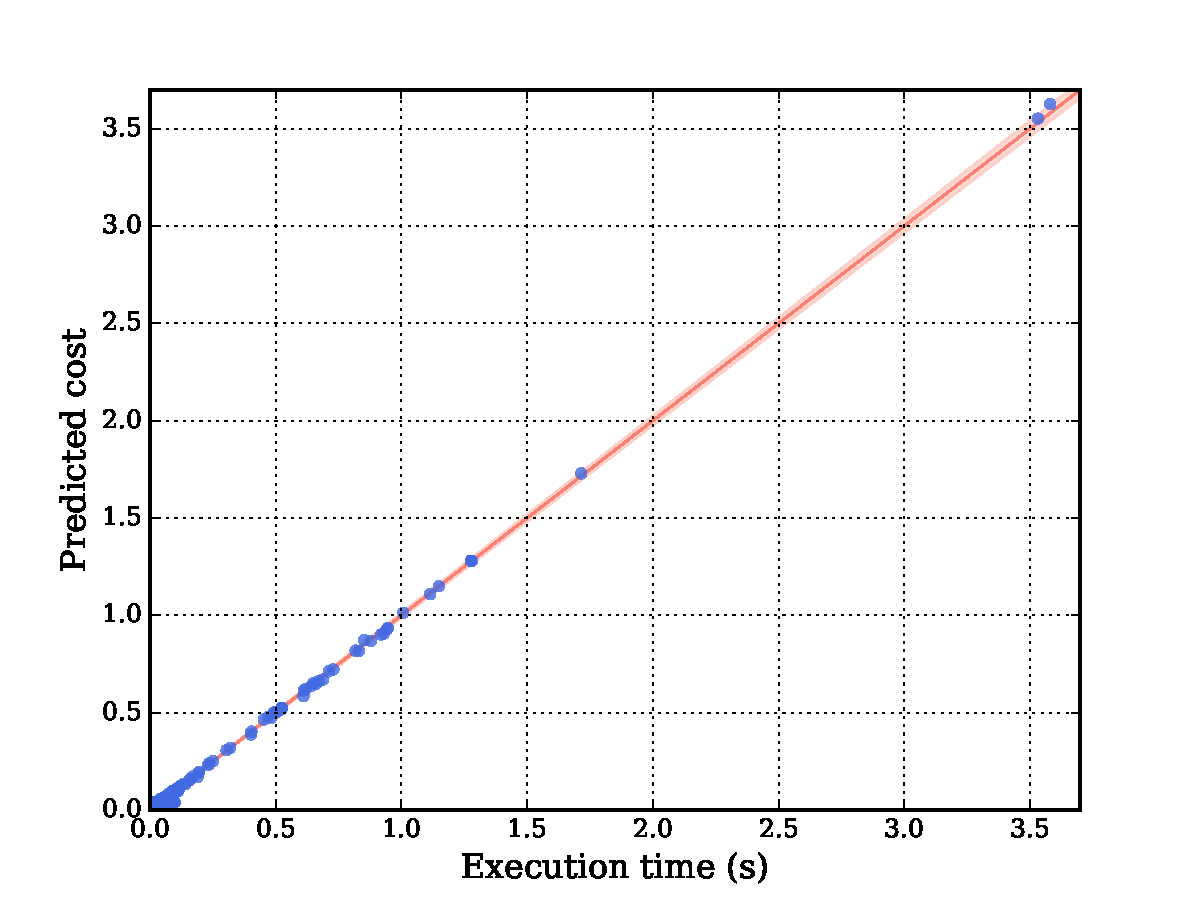
\includegraphics[width=0.6\linewidth]{figs/cost-model.pdf}
    %    \caption{
    %        Linear model for work metric fitted from empirical data.
    %        \red{zw: bigger font size.}
    %    }
    %    \label{fig:cost-model}
    %\end{figure}

    %\begin{figure}[t]
    %    \centering
    %    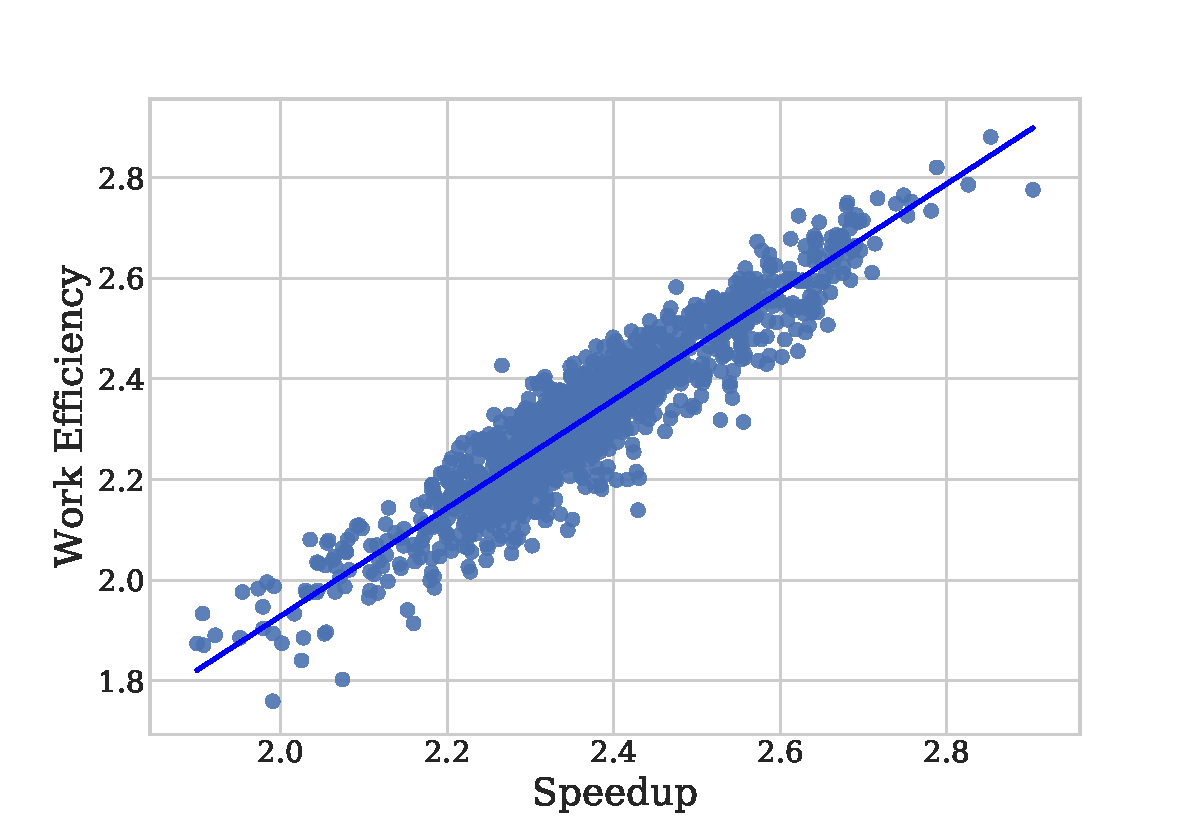
\includegraphics[width=0.5\textwidth]{figs/motivation-work-efficiency.pdf}
    %    \caption{Relationship between work efficiency \textit{vs} speedup for 500 different binaries of \texttt{susan\_c}.
    %            Each point represents the average over a subset of all inputs.
    %            The correlation coefficient is $0.93$.}
    %    \label{fig:motivation-work-efficiency}
    %\end{figure}
